\documentclass{beamer}
\usetheme{Boadilla}

\usepackage{graphicx}
\usepackage{subcaption}
\usepackage{csvsimple}

% Set relative path to all figures
\newcommand*{\floatRelativePath}{../out/gwas417/pval_5e-08/r2_0.1/kb_1000/window_1000000/75_50}%
% Footnote without marker: https://tex.stackexchange.com/questions/30720/footnote-without-a-marker
\newcommand\blfootnote[1]{%
    \begingroup
    \renewcommand\thefootnote{}\footnote{#1}%
    \addtocounter{footnote}{-1}%
    \endgroup
}
% Change size of footnotes
\renewcommand{\footnotesize}{\fontsize{5pt}{5pt}\selectfont}
% reset footnote counter for each frame in beamer class
\AtBeginEnvironment{frame}{\setcounter{footnote}{0}}

\title{Analysis of pleiotropy of eQTLs}
\subtitle{Internal Seminar}
\author{Aitor Gonz\'alez}
\institute{Aix Marseille Univ, INSERM, TAGC}
\date{Jan. 20, 2023}

% Add section slide
\AtBeginSection[]
{
    \begin{frame}
        \frametitle{Table of Contents}
        \tableofcontents[currentsection]
    \end{frame}
}

\begin{document}

%%%%%%%%%%%%%%%%%%%%%%%%%%%%%%%%%%%%%%%%%%%%%%%%%%%%%%%%%%%%%%%%%%%%%%%%%%%%%%%%
    \begin{frame}

        \titlepage

    \end{frame}

    \section{Introduction} %%%%%%%%%%%%%%%%%%%%%%%%%%%%%%%%%%%%%%%%%%%%%%%%%%%%%%%%%%%%%%

%%%%%%%%%%%%%%%%%%%%%%%%%%%%%%%%%%%%%%%%%%%%%%%%%%%%%%%%%%%%%%%%%%%%%%%%%%%%%%%%
%    The associations to diseases are heterougeneously distributed in the genome, Watanabe & Posthuma
%    This is based on loci associated to multiple traits
    \begin{frame}
        \frametitle{Genome-wide association studies (GWAS)}

        \begin{itemize}
            \item Association test of effect allele on case individuals
            \item High-throughput genetics: 3000 unique loci for over 250 disease/trait outcomes\footnote{Loos 2020. 10.1038/s41467-020-19653-5}
            \item Of the 1,707.0 Mb genome, 90.0\% is associated to different GWAS categories
        \end{itemize}
%
        \vfill
%          However, how do we know if these variants are active in a tissue,
%         or whether these variants false positives due to linkage disequilibrium,
%         or how these variants act molecularly
        Questions:
%
        \begin{itemize}
            \item Correlation between variants. Which is the causal variant?
            \item Which cell types important for disease?
            \item In which tissues are these variants active?
        \end{itemize}
%
        \vfill
%
        Questions partially addressed by looking at eQTLs in different tissues

        \blfootnote{}
        \blfootnote{Cano-Gamez et al. 2020. doi:10.3389/fgene.2020.00424}
    \end{frame}

%%%%%%%%%%%%%%%%%%%%%%%%%%%%%%%%%%%%%%%%%%%%%%%%%%%%%%%%%%%%%%%%%%%%%%%%%%%%%%%%
    \begin{frame}
        \frametitle{Expression quantitative trait loci (eQTLs)}

        \begin{columns}
            \begin{column}{0.5\textwidth}
                \begin{center}
                    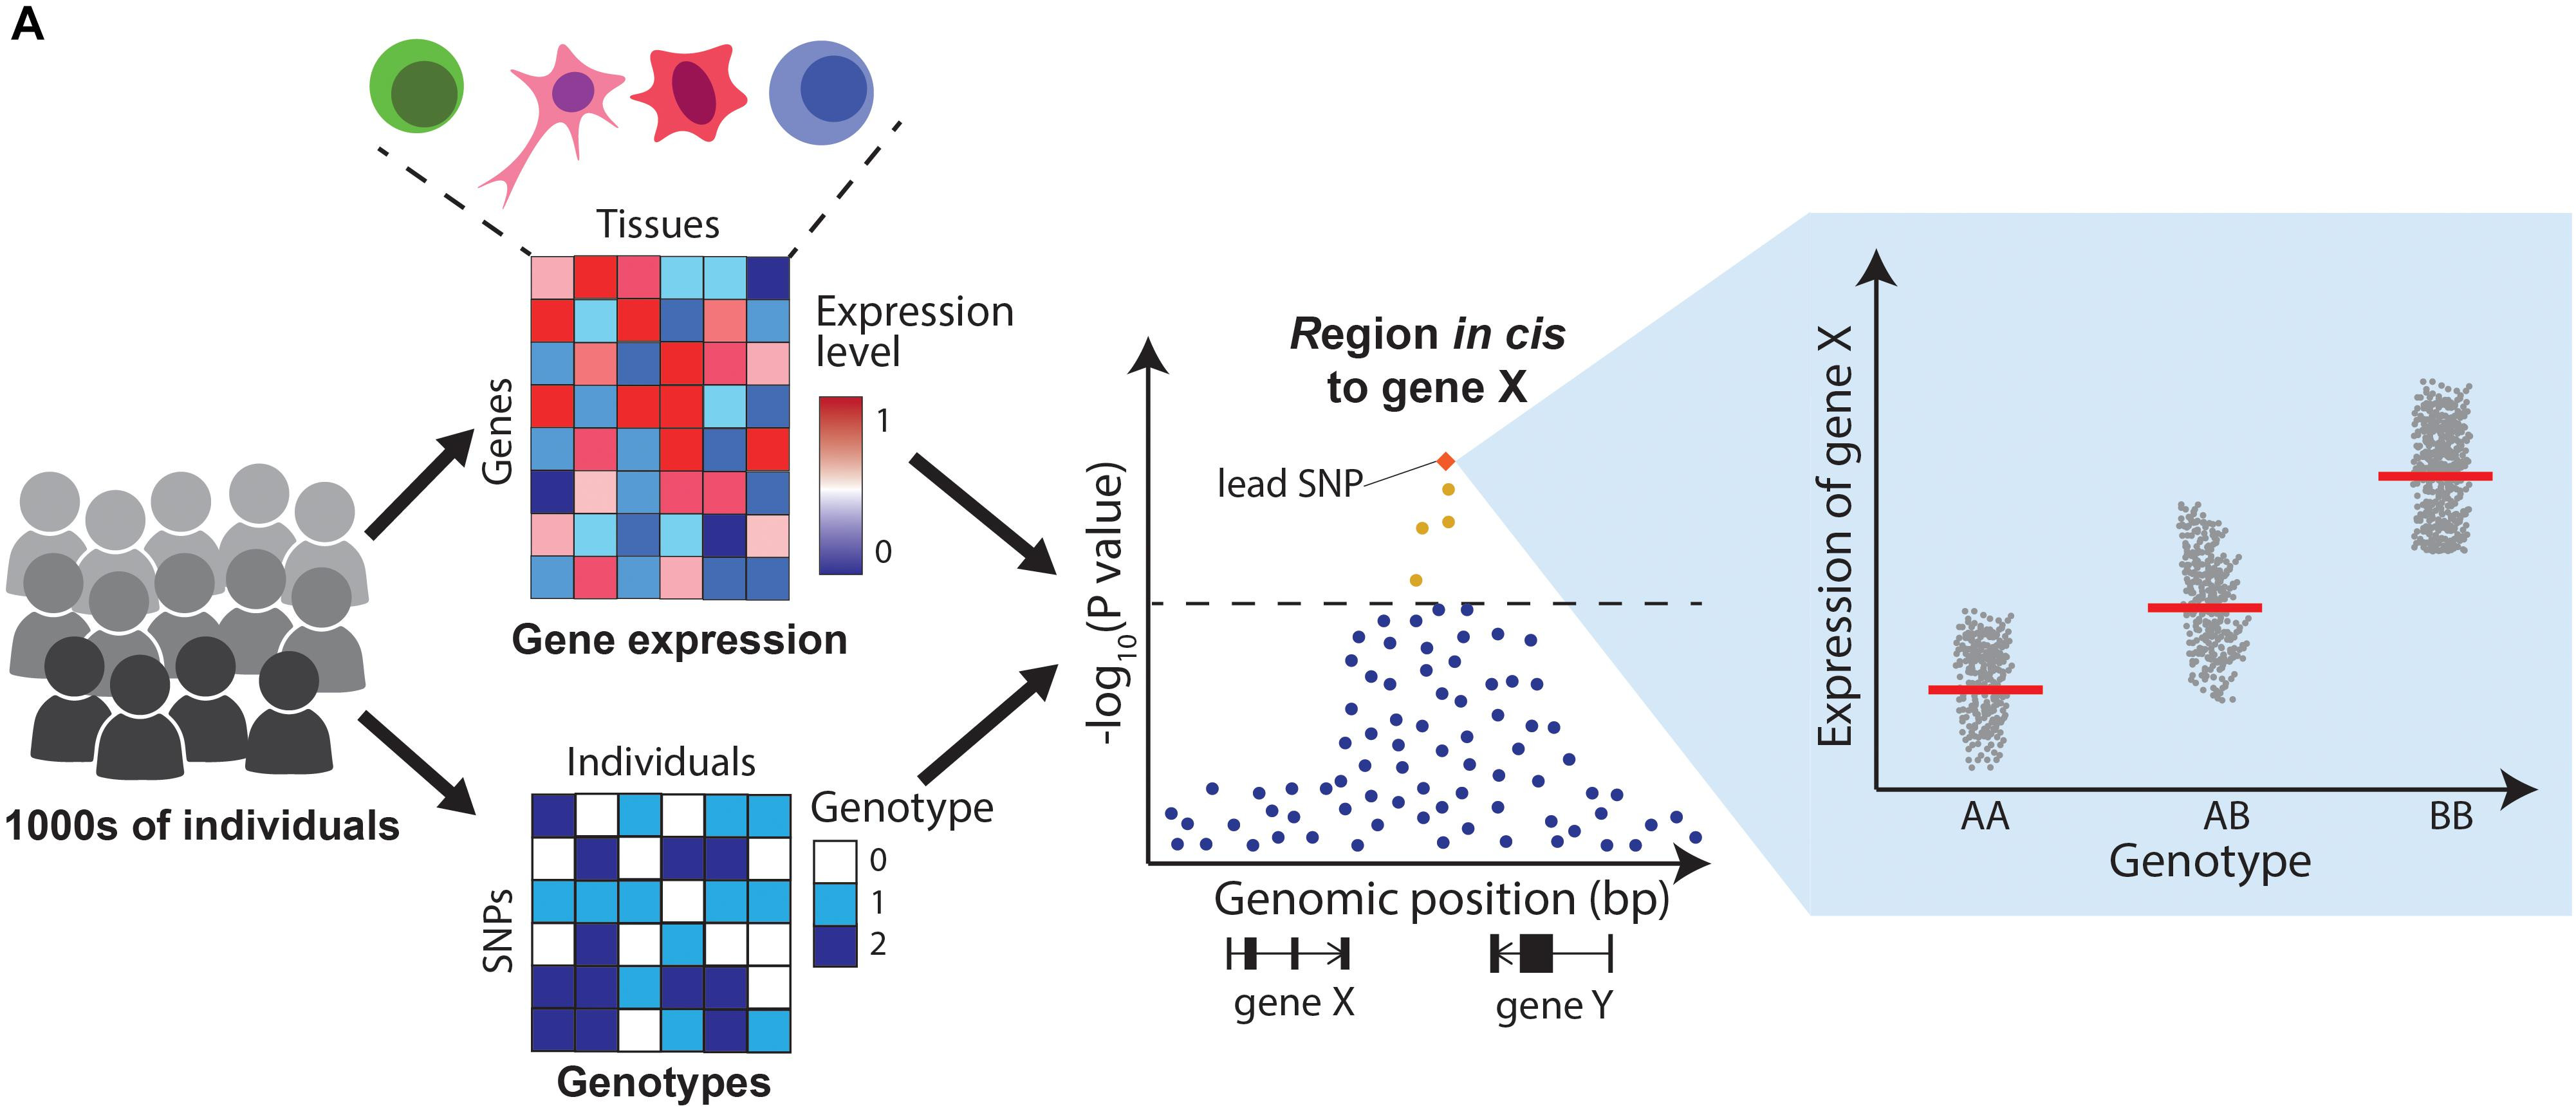
\includegraphics[width=\textwidth]{../presentation_230120_gold2022_paris/fig/doi_10.3389_fgene.2020.00424_fig4a.jpg}
                \end{center}
            \end{column}
            \begin{column}{0.5\textwidth}

            \end{column}
        \end{columns}

        \blfootnote{Cano-Gamez et al. 2020. doi:10.3389/fgene.2020.00424}
    \end{frame}

%%%%%%%%%%%%%%%%%%%%%%%%%%%%%%%%%%%%%%%%%%%%%%%%%%%%%%%%%%%%%%%%%%%%%%%%%%%%%%%%
    \begin{frame}
        \frametitle{Annotation of GWAS variants with gene and tissue targets using colocalization analysis}

        \begin{columns}
            \begin{column}{0.5\textwidth}
                \begin{center}
                    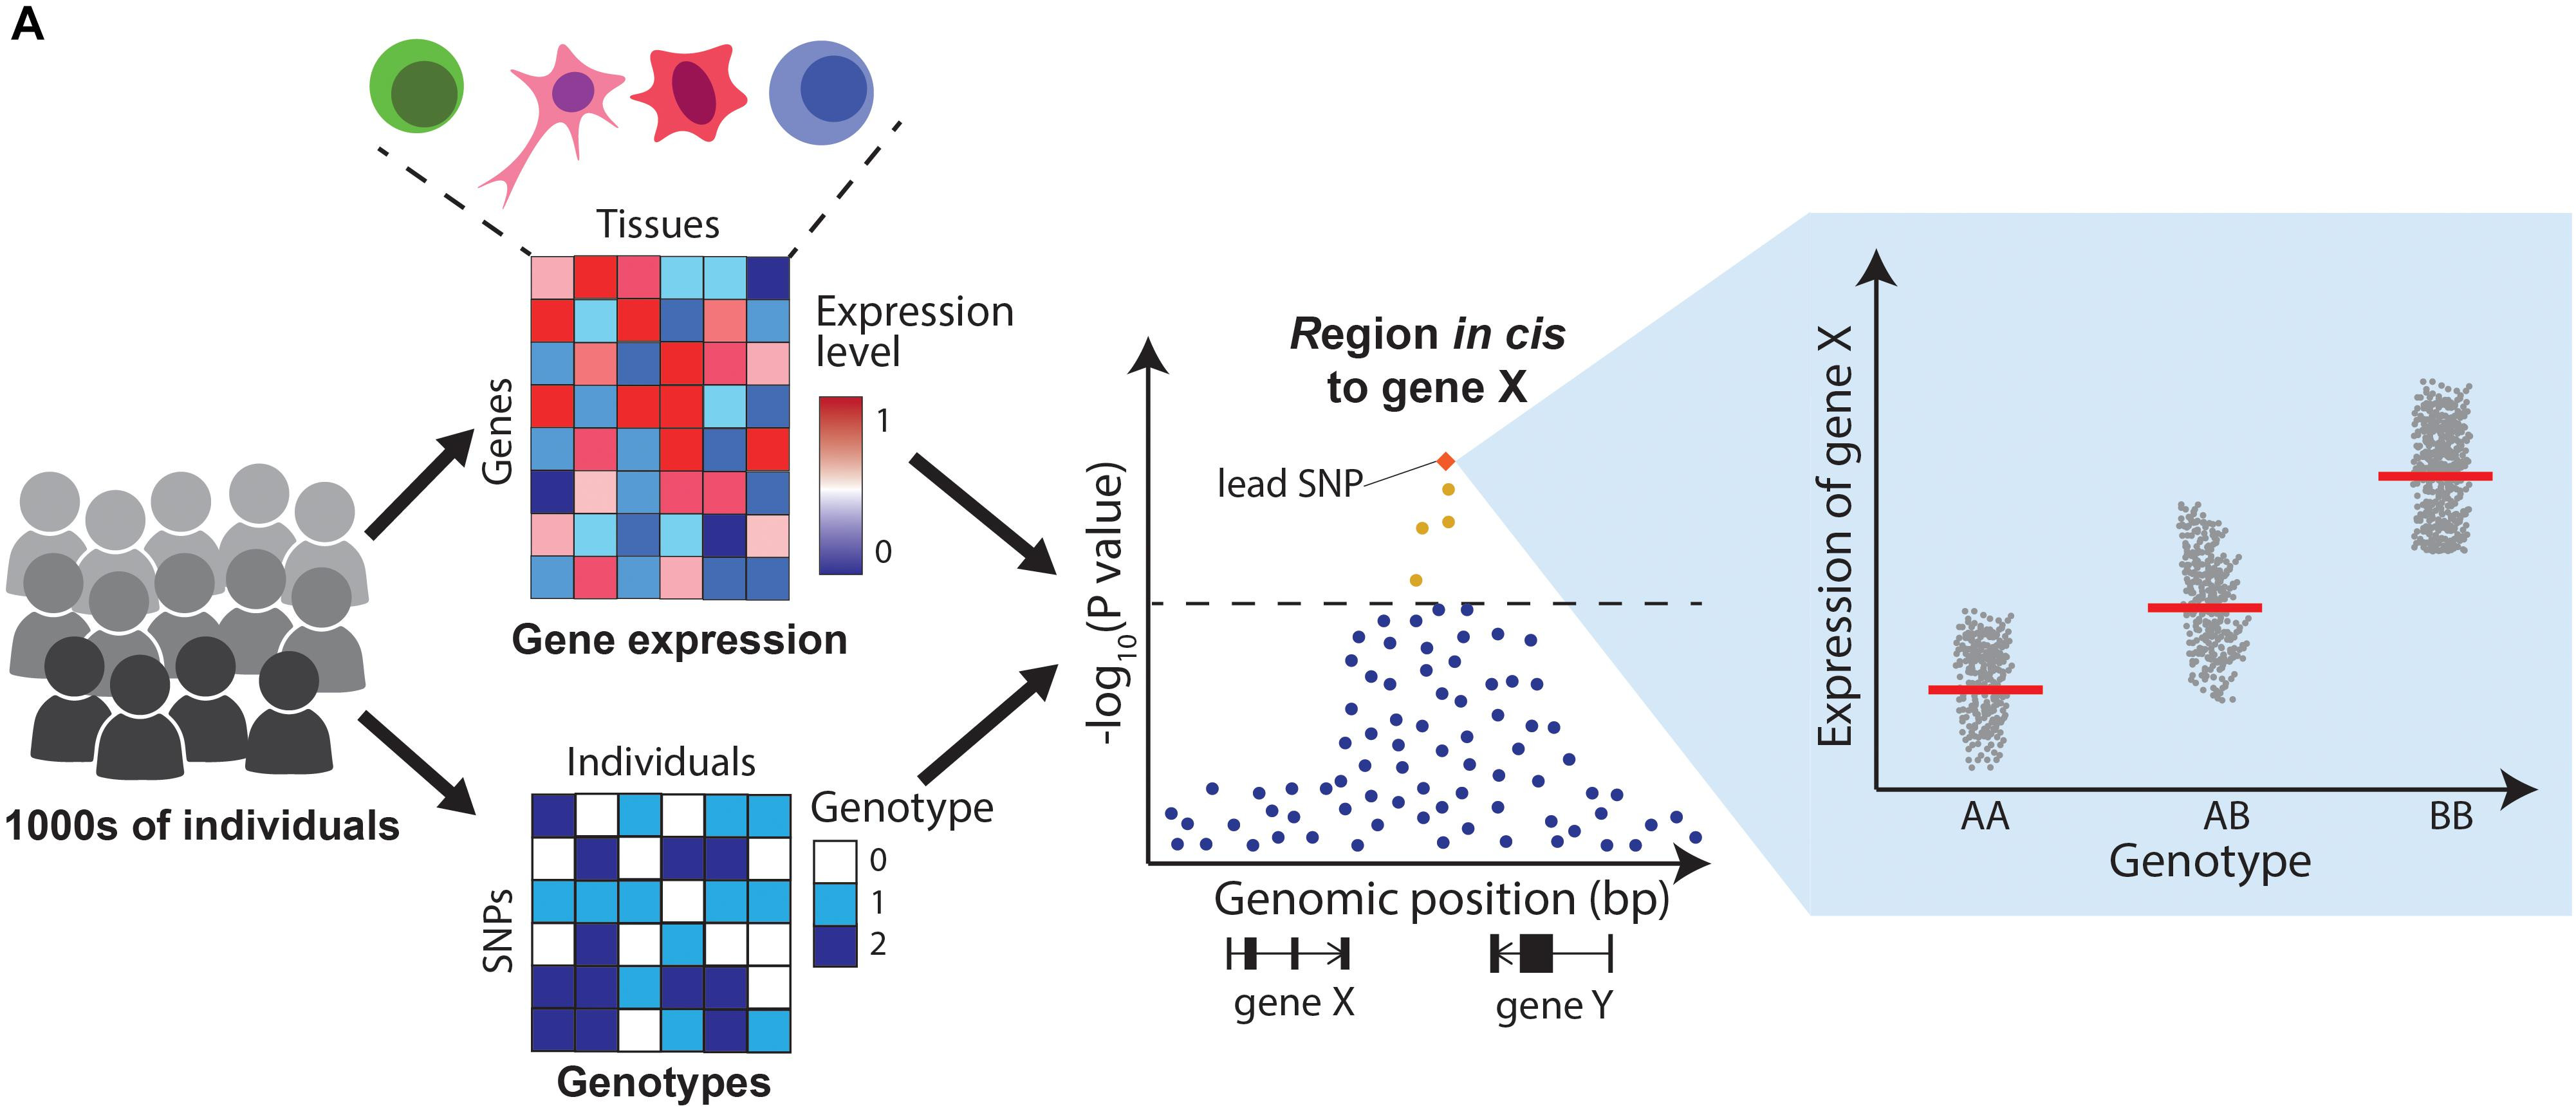
\includegraphics[width=\textwidth]{../presentation_230120_gold2022_paris/fig/doi_10.3389_fgene.2020.00424_fig4a.jpg}
                \end{center}
            \end{column}
            \begin{column}{0.5\textwidth}
                \begin{center}
                    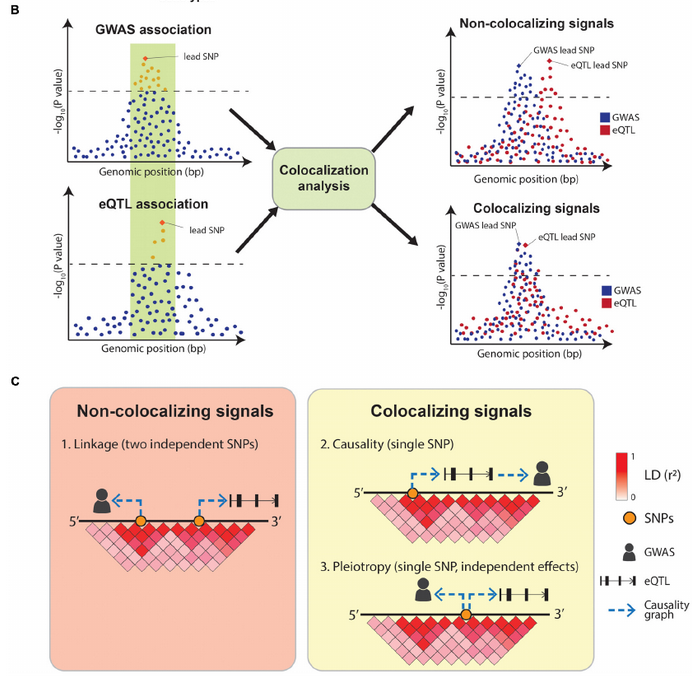
\includegraphics[width=\textwidth]{../presentation_230120_gold2022_paris/fig/doi_10.3389_fgene.2020.00424_fig4bc.png}
                \end{center}
            \end{column}
        \end{columns}

        \blfootnote{Cano-Gamez et al. 2020. doi:10.3389/fgene.2020.00424}
    \end{frame}

%%%%%%%%%%%%%%%%%%%%%%%%%%%%%%%%%%%%%%%%%%%%%%%%%%%%%%%%%%%%%%%%%%%%%%%%%%%%%%%%
    \begin{frame}
        \frametitle{Objectives}

        \begin{enumerate}
            \item Large scale gene and tissue annotation of variants of complex traits using GWAS/eQTL colocalization analysis
            \item To identify pleiotropic eQTLs and eQTL-containing genomic regions
            \item To characterize the properties of pleiotropic eQTLs
            \item To share colocalizations with experimentalists
        \end{enumerate}
    \end{frame}

%%%%%%%%%%%%%%%%%%%%%%%%%%%%%%%%%%%%%%%%%%%%%%%%%%%%%%%%%%%%%%%%%%%%%%%%%%%%%%%%
    \begin{frame}
        \frametitle{Data and Algorithms}

        \begin{columns}
            \begin{column}{0.5\textwidth}
                \begin{itemize}
                    \item IEA OpenGWAS database\footnote{https://gwas.mrcieu.ac.uk}: 418 GWAS datasets
                    \item EBI eQTLs database\footnote{https://www.ebi.ac.uk/eqtl}: Processed eQTLs from 127 studies in human.
                    \item CRAN - Package coloc\footnote{https://cran.r-project.org/web/packages/coloc/index.html}: Colocalisation analysis of GWAS/eQTL with one causal variant
                \end{itemize}
            \end{column}
            \begin{column}{0.5\textwidth}
                \begin{center}
                    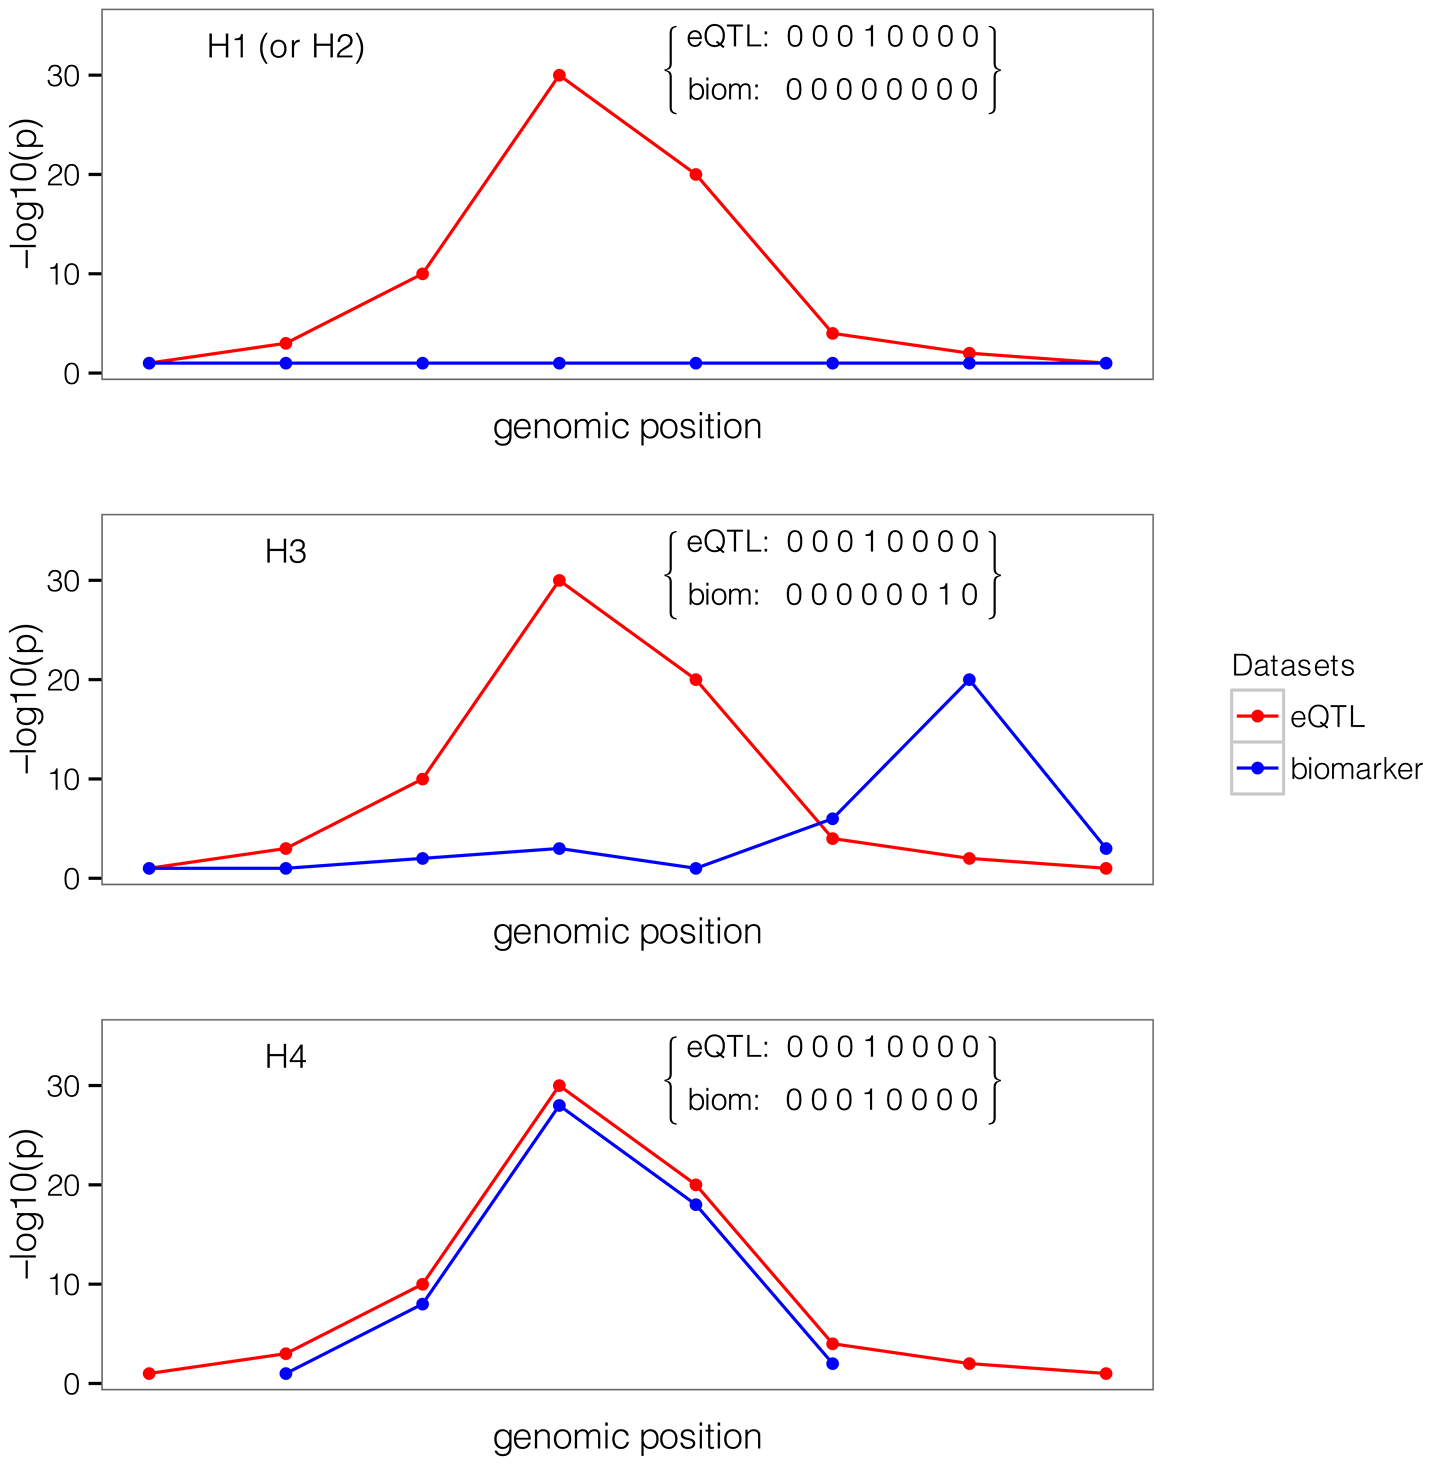
\includegraphics[width=\textwidth]{../presentation_230120_gold2022_paris/fig/pgen.1004383.g001.png}
                \end{center}
            \end{column}
        \end{columns}

%        \let\thefootnote\relax\footnotetext{$^1$https://gwas.mrcieu.ac.uk}
%        \let\thefootnote\relax\footnotetext{$^2$https://www.ebi.ac.uk/eqtl}
%        \let\thefootnote\relax\footnotetext{$^3$https://cran.r-project.org/web/packages/coloc/index.html}
    \end{frame}


    \section{Results}

%%%%%%%%%%%%%%%%%%%%%%%%%%%%%%%%%%%%%%%%%%%%%%%%%%%%%%%%%%%%%%%%%%%%%%%%%%%%%%%%
    \begin{frame}
        \frametitle{Large scale GWAS/eQTL colocalization analysis}

        \begin{itemize}
            \item Colocalization between 293 GWAS and 127 eQTL studies
            \item 138e3 colocalized variants with probability $\geq$ 0.75
            \item Percentage of GWAS loci explained by eQTL: 0$\%$ - 77$\%$ (Average 33$\%$)
        \end{itemize}

        \begin{figure}[!]
            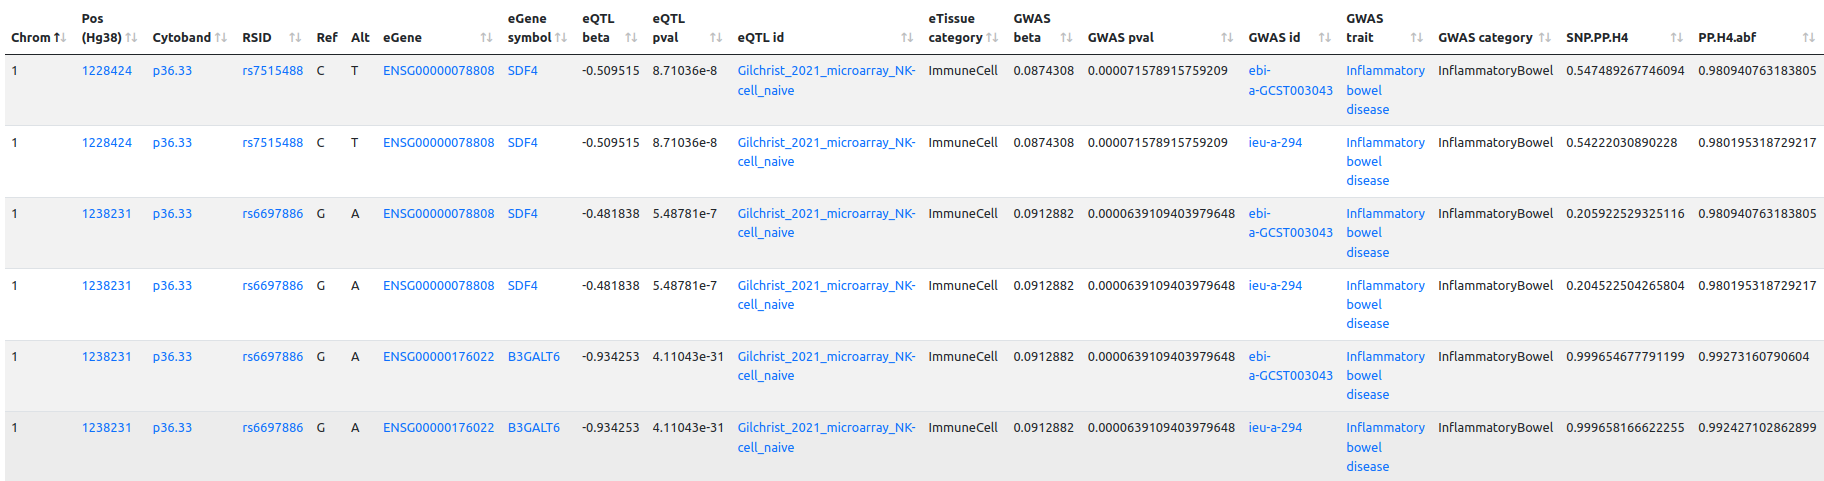
\includegraphics[width=\textwidth]{../presentation_230120_gold2022_paris/fig/coloc_web.png}
        \end{figure}

    \end{frame}

%%%%%%%%%%%%%%%%%%%%%%%%%%%%%%%%%%%%%%%%%%%%%%%%%%%%%%%%%%%%%%%%%%%%%%%%%%%%%%%%
    \begin{frame}
        \frametitle{Do GWAS traits cluster coherently?}

        GWAS distance based on correlation of beta of colocalized eQTL gene and tissue

        \begin{figure}[!]
            \includegraphics[width=0.5\textwidth]{\floatRelativePath/plthtmp_disease_comorbidity_matrix.py/corr_inkscape.png}
        \end{figure}

        \begin{itemize}
            \item Categories are coherent
            \item Help categorize GWAS traits
        \end{itemize}

    \end{frame}

%%%%%%%%%%%%%%%%%%%%%%%%%%%%%%%%%%%%%%%%%%%%%%%%%%%%%%%%%%%%%%%%%%%%%%%%%%%%%%%
%\begin{frame}
%\frametitle{Diseases?}
%
%\begin{table}[!tbp]
%\centering
%\scriptsize
%\hline
%\csvreader[separator=tab,
%tabular=ccrrp{0.4\textwidth},
%head,
%table head=\bfseries Chrom. & \bfseries Cytoband & \bfseries Pos (hg38) & \bfseries Variant & \bfseries GWAS Categories\\\hline,
%]{\floatRelativePath/cmpt_count_per_rsid.py/count_per_rsid_gwas_ms.tsv}{}% use head of csv as column names
%{\csvcoli\ & \csvcolii\ & \csvcoliii\ & \csvcoliv & \csvcolv}% specify your coloumns here
%\hline
%%
%\vspace{15pt}
%%
%\caption{Colocalized eQTL/GWAS variants involved in 5 or more GWAS categories. Genomic coordinates are given for the hg38 assembly. }\label{tab:pleitropic_variants}
%\end{table}
%
%\end{frame}

%%%%%%%%%%%%%%%%%%%%%%%%%%%%%%%%%%%%%%%%%%%%%%%%%%%%%%%%%%%%%%%%%%%%%%%%%%%%%%%%
    \begin{frame}
        \frametitle{How are pleiotropic eQTLs defined?}

        \begin{itemize}
            \item Uniformly annotate GWAS traits based on clustering and EBI ontologies
            \item Aggregate colocalised eQTLs based on the number of trait categories
            \item Analyse eQTLs in groups based on the number of trait categories
        \end{itemize}

    \end{frame}

    %%%%%%%%%%%%%%%%%%%%%%%%%%%%%%%%%%%%%%%%%%%%%%%%%%%%%%%%%%%%%%%%%%%%%%%%%%%%%%%%
    \begin{frame}
        \frametitle{Winner (Most pleiotroic) eQTLs?}

        \begin{itemize}
            \item Example eQTLs involved in four GWAS categories in different cytobands
            \item The gene marker is the eQTL gene with the highest PubMed publication count
        \end{itemize}

% full size table is table
        \begin{table}[!tbp]
            \centering
            \footnotesize
            \csvreader[separator=tab,
            tabular=crclcp{0.4\textwidth},
            head,
            table head=\bfseries Chrom. & \bfseries Pos (hg38) & \bfseries Cytoband & \bfseries RSID & \bfseries Known eQTL gene & \bfseries GWAS Categories\\\hline,
            ]{\floatRelativePath/cmpt_count_per_rsid.py/count_per_rsid_gwas_ms.tsv}{}% use head of csv as column names
                {\csvcoli\ & \csvcolii\ & \csvcoliii\ & \csvcoliv\ & \csvcolv\ & \csvcolvi}% specify your coloumns here
            \vspace{15pt}
        \end{table}

    \end{frame}

    %%%%%%%%%%%%%%%%%%%%%%%%%%%%%%%%%%%%%%%%%%%%%%%%%%%%%%%%%%%%%%%%%%%%%%%%%%%%%%%%
    \begin{frame}
        \frametitle{Winner (Most pleiotroic) regions?}

% full size table is table
        \begin{table}[!tbp]
            \centering
            \footnotesize
%\hline
            \csvreader[
                separator=tab,
                tabular=p{0.005\textwidth}p{0.05\textwidth}p{0.05\textwidth}p{0.05\textwidth}p{0.05\textwidth}p{0.5\textwidth},
                head,
                table head=\bfseries Chr. & \bfseries Start & \bfseries End & \bfseries Cytob. & \bfseries Known eQTL gene & \bfseries GWAS Categories\\\hline,
            ]{\floatRelativePath/cmpt_pleiotropic_regions.py/100000/region_window_ms.tsv}{}% use head of csv as column names
            {\csvcoli\ & \csvcolii\ & \csvcoliii\ & \csvcoliv\ & \csvcolv\ & \csvcolvi}% specify your coloumns here
%\hline
%
            \vspace{15pt}
            \caption{Pleiotropic regions involving 6 or more GWAS classes. These regions were built with a sliding window of 1e5 nt. Genomic coordinates are given for the hg38 assembly.}\label{tab:pleiotropic_regions}
        \end{table}

    \end{frame}

%%%%%%%%%%%%%%%%%%%%%%%%%%%%%%%%%%%%%%%%%%%%%%%%%%%%%%%%%%%%%%%%%%%%%%%%%%%%%%%%%
%\begin{frame}
%    \frametitle{How are pleiotropic variants distributed?}
%
%    \begin{columns}
%        \begin{column}{0.32\textwidth}
%            \begin{center}
%                \includegraphics[width=\textwidth]{\floatRelativePath/pltsctr_x_per_rsid_y_gwas.py/count_per_rsid_chr5_start131912097_end132802472_categories7.png}
%            \end{center}
%        \end{column}
%        \begin{column}{0.32\textwidth}
%            \begin{center}
%                \includegraphics[width=\textwidth]{\floatRelativePath/pltsctr_x_per_rsid_y_egene.py/count_per_rsid_chr5_start131912097_end132802472_categories7.png}
%            \end{center}
%        \end{column}
%        \begin{column}{0.32\textwidth}
%            \begin{center}
%                \includegraphics[width=\textwidth]{\floatRelativePath/pltsctr_x_per_rsid_y_etissue.py/count_per_rsid_chr5_start131912097_end132802472_categories7.png}
%            \end{center}
%        \end{column}
%    \end{columns}
%
%    \begin{center}
%        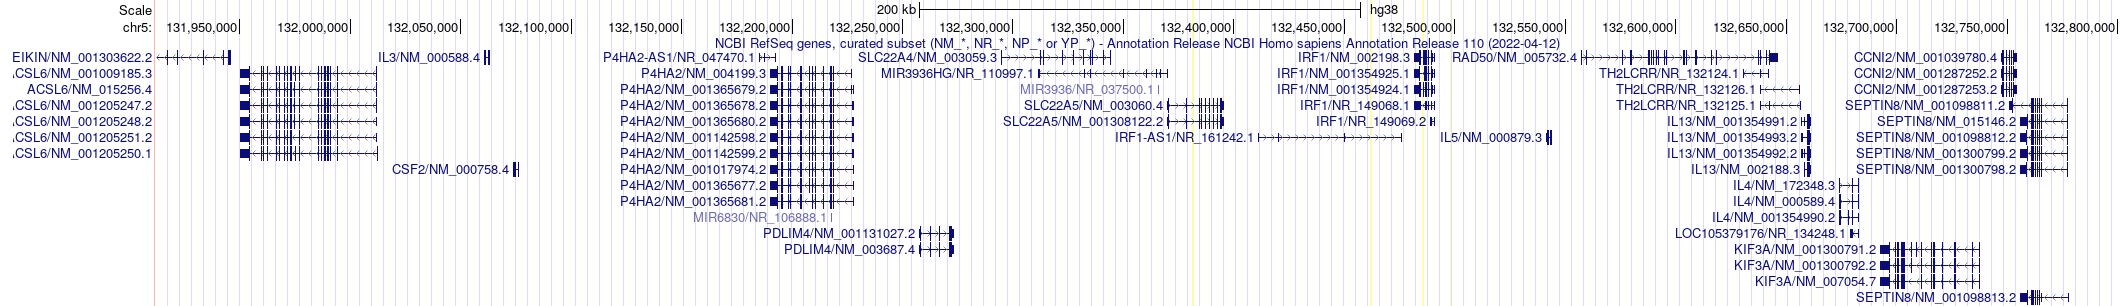
\includegraphics[width=\textwidth]{../presentation_230120_gold2022_paris/fig/chr5_131912097_132802472.png}
%    \end{center}
%
%    \small
%    \begin{itemize}
%        \item The cytokine locus: chr5:131,912,097-132,802,472. Genes IRF1, IL3, IL4, IL5, ...
%        \item Diseases: Allergy,Autoimmune dis.,Cancer of breast,Circulatory sys. dis.,Hypertension,Respiratory system dis.
%        \item For instance: rs2522051 regulates 12 e-genes in 23 e-tissues
%    \end{itemize}
%    \normalsize
%
%\end{frame}

%%%%%%%%%%%%%%%%%%%%%%%%%%%%%%%%%%%%%%%%%%%%%%%%%%%%%%%%%%%%%%%%%%%%%%%%%%%%%%%%
    \begin{frame}
        \frametitle{Where are the pleiotropic variants?\footnote{https://www.ensembl.org/vep}}

        \begin{center}
            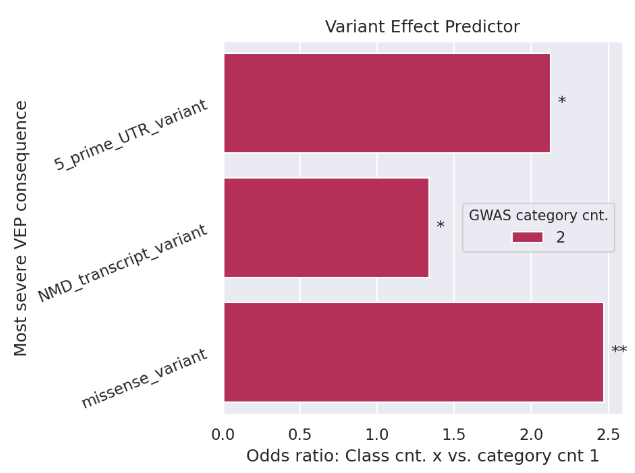
\includegraphics[width=0.7\textwidth]{\floatRelativePath/pltbar_vep_consequence.py/vep.png}
        \end{center}

        In the transcripts

%        \let\thefootnote\relax\footnotetext{$^1$https://www.ensembl.org/vep}

    \end{frame}

%%%%%%%%%%%%%%%%%%%%%%%%%%%%%%%%%%%%%%%%%%%%%%%%%%%%%%%%%%%%%%%%%%%%%%%%%%%%%%%%
    \begin{frame}
        \frametitle{Do pleiotropic variants associate to more eQTL genes?}

        \begin{columns}
            \begin{column}{0.5\textwidth}
                \begin{center}
                    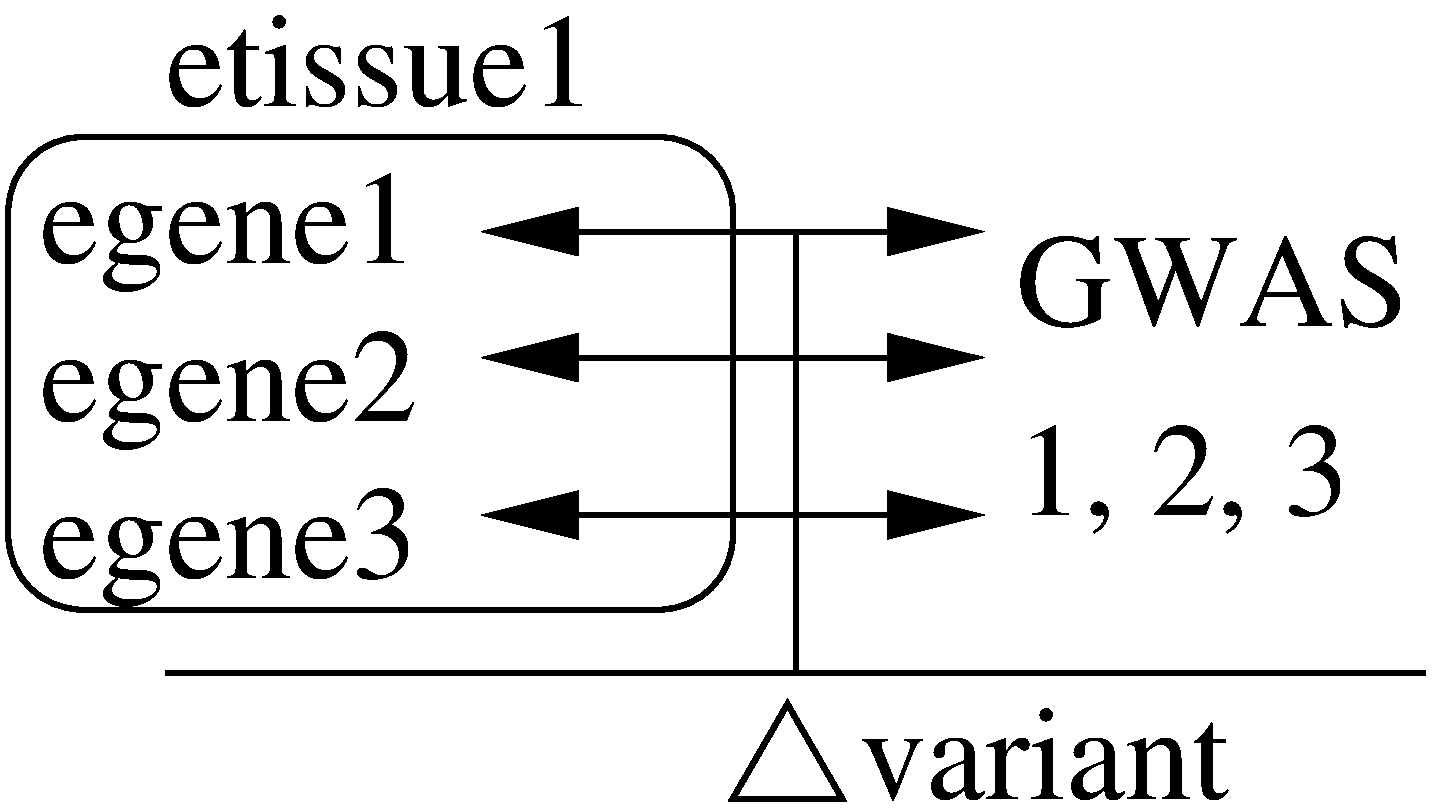
\includegraphics[width=0.7\textwidth]{../presentation_230120_gold2022_paris/fig/model_pleio_egenes.png}
                \end{center}
            \end{column}
            \begin{column}{0.5\textwidth}  %%<--- here
                \begin{center}
                    \includegraphics[width=\textwidth]{\floatRelativePath/pltbar_x_per_variant_etissue_y_egene.py/plt.png}
                \end{center}
            \end{column}
        \end{columns}

    \end{frame}

%%%%%%%%%%%%%%%%%%%%%%%%%%%%%%%%%%%%%%%%%%%%%%%%%%%%%%%%%%%%%%%%%%%%%%%%%%%%%%%%
    \begin{frame}
        \frametitle{Do pleiotropic variants associate to more eQTL tissues?}

        \begin{columns}
            \begin{column}{0.5\textwidth}
                \begin{center}
                    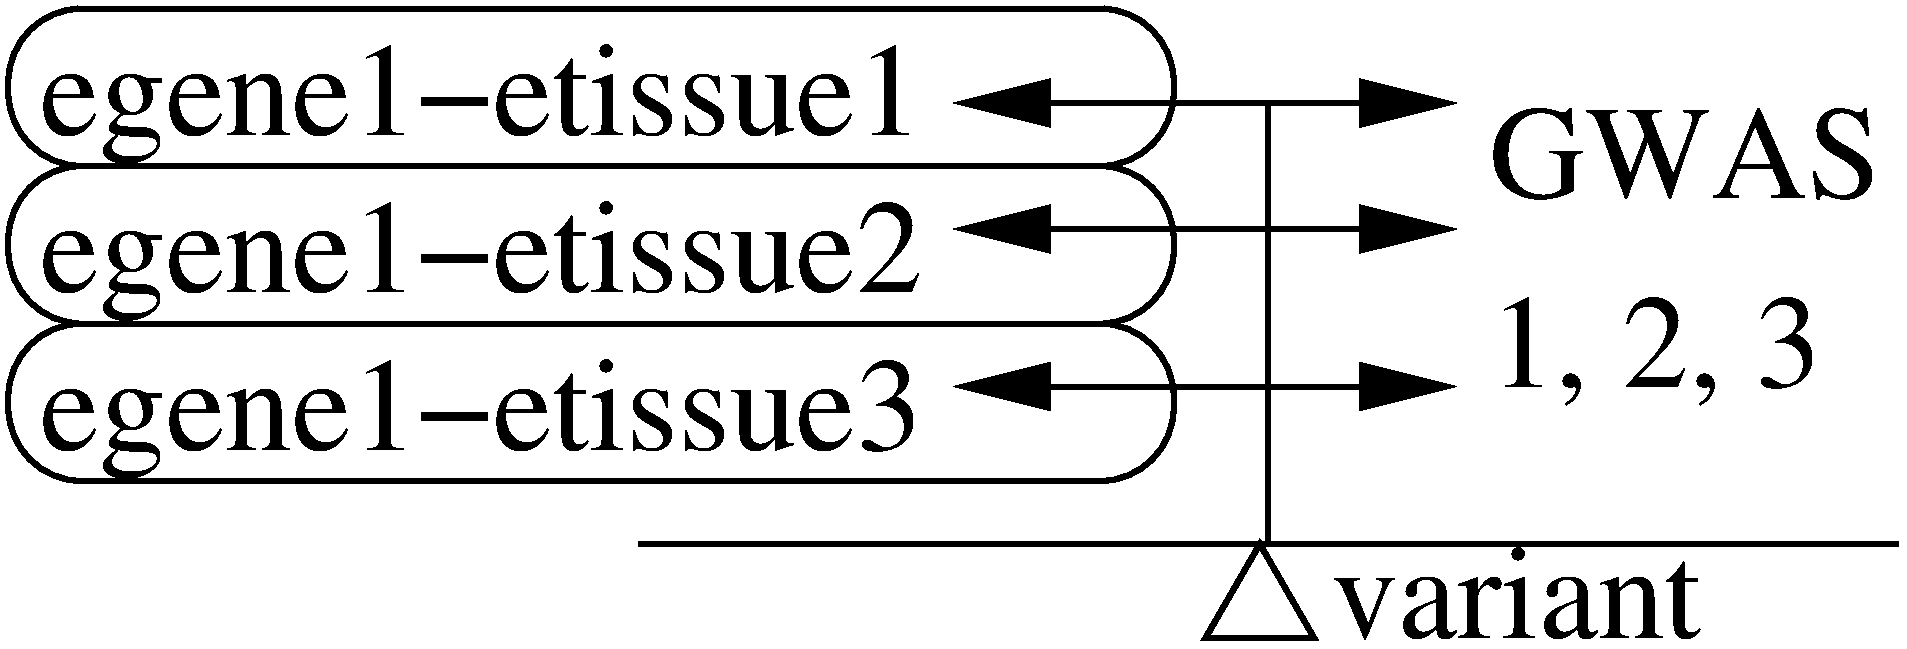
\includegraphics[width=0.7\textwidth]{../presentation_230120_gold2022_paris/fig/model_pleio_etissues.png}
                \end{center}
            \end{column}
            \begin{column}{0.5\textwidth}  %%<--- here
                \begin{center}
                    \includegraphics[width=\textwidth]{\floatRelativePath/pltbar_x_per_variant_egene_y_etissue.py/plt.png}
                \end{center}
            \end{column}
        \end{columns}

    \end{frame}

%%%%%%%%%%%%%%%%%%%%%%%%%%%%%%%%%%%%%%%%%%%%%%%%%%%%%%%%%%%%%%%%%%%%%%%%%%%%%%%%
    \begin{frame}
        \frametitle{Do pleiotropic variants bind more transcription factors?\footnote{https://remap.univ-amu.fr}}

        \begin{columns}
            \begin{column}{0.5\textwidth}
                \begin{center}
                    \includegraphics[width=\textwidth]{\floatRelativePath/pltbox_x_per_rsid_y_remapnr.py/bxplt_remaptf_per_rsid_flank_10.png}
                \end{center}
            \end{column}
            \begin{column}{0.5\textwidth}  %%<--- here
                \begin{center}
                    \includegraphics[width=\textwidth]{\floatRelativePath/pltbar_x_per_variant_pleiotropy_y_remapcrm.py/remapcrm_flank10.png}
                \end{center}
            \end{column}
        \end{columns}

%        \let\thefootnote\relax\footnotetext{$^1$https://remap.univ-amu.fr}

    \end{frame}

    \section{Conclusions, perspective and acknowledgements} %%%%%%%%%%%%%%%%%%%%%%%%%%%%%%%%%%%%%%%%%%%%%%%%%%%%%%%%%%%%%%

%%%%%%%%%%%%%%%%%%%%%%%%%%%%%%%%%%%%%%%%%%%%%%%%%%%%%%%%%%%%%%%%%%%%%%%%%%%%%%%%
    \begin{frame}
        \frametitle{Concluding remarks}

        Outcomes interesting for the GOLD population genotypes
%
        \begin{itemize}
            \item A large set of causal GWAS variants annotated with target genes and tissues
            \item A list of pleiotropic variants and regions
        \end{itemize}
%
        \vfill
%
        What are the gene regulatory properties underlying pleiotropy between complex traits?
%
        \begin{itemize}
            \item Variant pleiotropy is correlated in regions
            \item Enrichment of variants upstream (incl. 5'UTR) and downstream of genes (incl. 3'UTR)
            \item Enrichment of transcription factor and CRM binding
            \item Increased number of associated egenes and etissues
        \end{itemize}


    \end{frame}

%%%%%%%%%%%%%%%%%%%%%%%%%%%%%%%%%%%%%%%%%%%%%%%%%%%%%%%%%%%%%%%%%%%%%%%%%%%%%%%%
    \begin{frame}
        \frametitle{Perspectives}


        \begin{itemize}
            \item A web portail to share data
            \item Causality of eQTL genes on GWAS (Looking for experts ;-) )
        \end{itemize}

    \end{frame}

%%%%%%%%%%%%%%%%%%%%%%%%%%%%%%%%%%%%%%%%%%%%%%%%%%%%%%%%%%%%%%%%%%%%%%%%%%%%%%%%
    \begin{frame}
        \frametitle{Acknowledgements}

        \begin{itemize}
            \item L\'eopoldine Lecerf (M1)
            \item P Paul, P Rihet, M Michel, S Marquet, S Spicuglia
        \end{itemize}
%
        \vfill
%
        Funding
%
        \begin{itemize}
            \item Institut Cancer et Immunologie - Aix-Marseille Univ.
            \item Agence nationale de la recherche (ANR)
            \item GOLD
        \end{itemize}

    \end{frame}

%%%%%%%%%%%%%%%%%%%%%%%%%%%%%%%%%%%%%%%%%%%%%%%%%%%%%%%%%%%%%%%%%%%%%%%%%%%%%%%%
    \begin{frame}
        \frametitle{}

    \end{frame}

%%%%%%%%%%%%%%%%%%%%%%%%%%%%%%%%%%%%%%%%%%%%%%%%%%%%%%%%%%%%%%%%%%%%%%%%%%%%%%%%
%\begin{frame}
%    \frametitle{Do pleiotropic variants associate to more traits (after fixing egene-etissue)?}
%
%    \begin{columns}
%        \begin{column}{0.5\textwidth}
%            \begin{center}
%                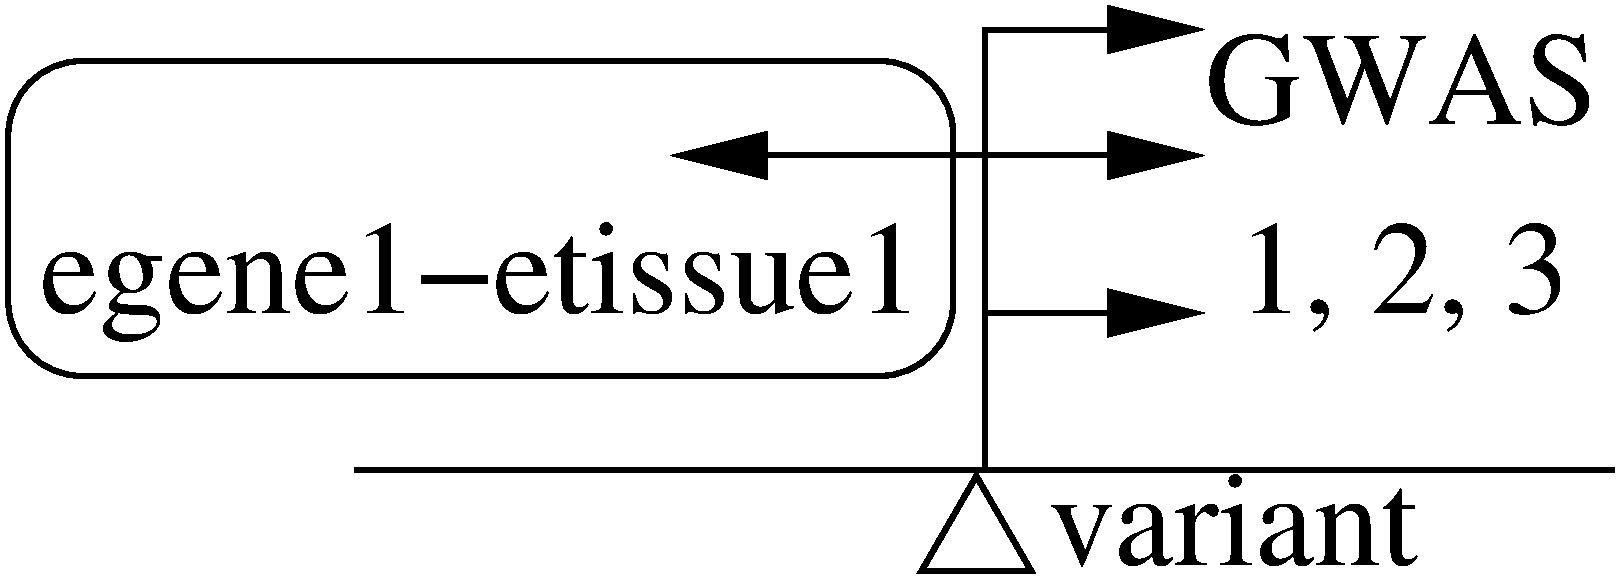
\includegraphics[width=0.7\textwidth]{../presentation_230120_gold2022_paris/fig/model_pleio_gwas.png}
%            \end{center}
%        \end{column}
%        \begin{column}{0.5\textwidth}  %%<--- here
%            \begin{center}
%                \includegraphics[width=\textwidth]{\floatRelativePath/pltbar_x_per_variant_egene_etissue_y_gwas.py/plt.png}
%            \end{center}
%        \end{column}
%    \end{columns}
%
%\end{frame}

\end{document}


